\documentclass[letterpaper,12pt]{article}
\usepackage[utf8]{inputenc}
\usepackage[spanish,ngerman]{babel}
\selectlanguage{ngerman}
\usepackage[rmargin=2cm, lmargin=1.5cm, tmargin= 2.8cm, bmargin=2.8cm]{geometry}
\usepackage[svgnames,x11names,dvipsnames]{xcolor} 
\usepackage{graphics}
\usepackage[rightcaption]{sidecap}
\usepackage{caption}
\usepackage{mathrsfs}
\usepackage{amssymb}
\usepackage{amsmath}
\usepackage{mathrsfs}
\usepackage{dsfont}
\usepackage{array}
\usepackage{amsfonts}
\usepackage{xcolor}
\usepackage{latexsym} %permite 
\usepackage{graphicx}
\usepackage{multirow}
\usepackage{wrapfig}
\usepackage{multicol}
\usepackage{multirow}
\usepackage{hyperref}
\usepackage{biblatex}%para las bibliografias

\newenvironment{Figura}
{\par\medskip\noindent\minipage{\linewidth}}
  {\endminipage\par\medskip}


%---------COLORES--------------------
\definecolor{azulito}{RGB}{40, 190, 188}
\definecolor{r0jo}{RGB}{190, 40, 74}
\definecolor{v3rd3}{RGB}{83, 190, 40}
\definecolor{amarill0}{RGB}{190, 183, 40 }

\pagecolor{white} %color a la hoja
\color{black} %color de letra

%http://latexcolor.com/ 

%-----------CABECERA-----------------
\usepackage{fancyhdr}%paqueteria para modificar encabezados
\pagestyle{headings} %cabecera 
\pagestyle{fancy} %pone la paqueteria
    \rfoot{página \thepage}
    \cfoot{}
    \lfoot{Méndez González Romina Estephania}
%---------------------------------



\begin{document}

\begin{center}
    \textbf{\Large{Tarea 5 - Problemas físicos}}
\end{center}


\section{Problemas}
\begin{enumerate}
    \item Considerando un sistema en una dimensión y sabiendo que $a=\tfrac{dv}{dt}$ y $v=\tfrac{dx}{dt}$. Demuestre que la posición se puede ver como:
    \begin{equation}
        x =x_{0} + v_{0}t+ \frac{1}{2}at^2
    \end{equation}
    Para un tiempo inicial $t_0 = 0$ y con; $x_0$ y $v_0$ la posición y velocidad inicial en el sistema.
\subsection*{Dem.}
Partiendo de que $a=\tfrac{dv}{dt}$, es claro que $a dt=dv$. Por lo que si integramos ambos lados de $a dt=dv$, o lo que es lo mismo  $dv=a dt$, obtenemos:
    \begin{equation}
        \int_{t}^{t_0} a dt= \int_{v_0}^{v} dv
    \end{equation}
Si $a$ es constante, entonces podemos sacarla de la integral y de (2) se sigue que:
    \begin{equation}
        a \int_{t}^{t_0} dt= \int_{v_0}^{v} dv 
    \end{equation}
De (3) se sigue que:
    \begin{equation}
        a t \Big|_{t_0}^t = v \Big|_{v_0}^v
    \end{equation}
Evaluando los límites de integración de (4) y tomando en cuenta que $t_0 = 0$, se obtiene:
    \begin{equation}
        at = v - v_0
    \end{equation}
Despejando a $v$ de (5):
    \begin{equation}
        v = v_0 + at
    \end{equation}
Ahora bien, como $v=\tfrac{dx}{dt}$, al igualar esta expresión con (6) se tiene que:
    \begin{equation}
        \frac{dx}{dt} = v_0 + at
    \end{equation}
Despejando de (7) al diferencial de x:
    \begin{equation}
        dx = (v_0 + at) dt
    \end{equation}
Integrando ambos lados de (8):
    \begin{equation}
        \int_{x}^{x_0} dx = \int_{t_0}^{t} (v_0 + at) dt 
    \end{equation}
Por propiedades de la integral, dado que abre sumas, de (9) tenemios que:
    \begin{equation}
        \int_{x}^{x_0} dx = \int_{t_0}^{t} v_0 dt +  \int_{t_0}^{t}at dt 
    \end{equation}
Como $a$ es constante al igual que $v_0$, entonces salen de la integral:
    \begin{equation}
        \int_{x}^{x_0} dx = v_0\int_{t_0}^{t} dt +  a\int_{t_0}^{t}t dt 
    \end{equation}
Resolviendo las integrales de (11):
    \begin{equation}
        x\Big|_{x_0}^x = v_{0}t \Big|_{t_0}^t + a (\tfrac{1}{2}t^2)\Big|_{t_0}^t
    \end{equation}
Evaluando (12) en sus respectivos límites de integración:
    \begin{equation}
        (x-x_0) = v_{0}(t - t_0) + a \tfrac{1}{2}(t-t_0)^2= v_{0}(t - t_0) +  \tfrac{1}{2}a(t-t_0)^2
    \end{equation}
Finalmente, sabemos que $t_0=0$, por lo que al sustituir el valor en (13) y despejando a $x$, obtenemos:
    \begin{equation}
        x = x_0 + v_{0}t + a\tfrac{1}{2}(t-t_0)^2
    \end{equation}
\hspace{16.5cm}$\blacksquare$

%-------------------------PROBLEMA 2--------------------------
    \item Considere una carrera entre dos coches, éstos arrancan del reposo pero el coche uno hace trampa (cosa que nunca pasa), saliendo un segundo antes que el segundo, si los autos tienen una aceleración de $3.5 \frac{m}{s^2}$ y $4.9 \frac{m}{s^2}$ respectivamente.
    \begin{enumerate}
        \item En qué momento el auto dos alcanza al auto uno, i.e. t =?
        \item Cuál será la posición cuando el inciso (a) ocurra, x =?
        \item Cuál será la velocidad que tendrá en ese punto para ambos autos
        \item Toma 5 tiempos diferentes a partir de que los autos arrancan, sin tomar el tiempo inicial, 3 antes del tiempo donde los autos se encuentran y dos posteriores a ese tiempo, realicen dos tablas, una para cada auto, con la siguiente información; aceleración, tiempo, posición y velocidad como se muestra en el Cuadro 1.
    \end{enumerate}
\subsection*{Solución a)}
Para la solución de este problema, haremos uso del siguiente diagrama:\\
    \begin{figure}
        \centering
        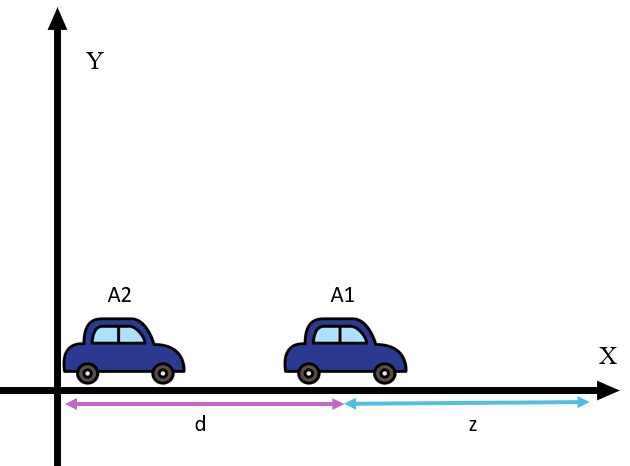
\includegraphics[scale=0.45]{Imagenes/Autos.png}
        \caption{Diagrama de la situación}
        \label{fig:my_label}
    \end{figure}
\underline{Obs.} Nótese que para que el auto 2 se encuentre con el auto 1, éste debe recorrer un desplazamiento igual a $d+z$, mientras que el auto 2 solo recorrerá un desplazamiento igual a $z$. \\
Así pues, el problema nos da los siguientes datos: $v_{0_{A1}}=0\frac{m}{s}$, $v_{0_{A2}}=0\frac{m}{s}$, $a_{A1}=3.5 \frac{m}{s^2}$, $a_{A2}=4.9 \frac{m}{s^2}$, $t_{A1}= 1s$. \\ \\
La ecuación cinemática que relaciona el desplazamiento, la aceleración y el tiempo es:
$$x= v_0 t + \tfrac{1}{2}a t^2$$
Sin embargo, como la velocidad inicial en ambos autos es igual a cero, nos conviene usar:
\begin{equation}
    x=  \tfrac{1}{2}a t^2
\end{equation}
De la observación antes mencionada y de (15), obtenemos las siguientes igualdades:
\begin{equation}
    d+ z= \tfrac{1}{2}a_{A2} t^2 
\end{equation}
\begin{equation}
    z= \tfrac{1}{2}a_{A1} t^2  
\end{equation}
Sustituyendo (17) en (16) nos queda:
\begin{equation}
    d+ \tfrac{1}{2}a_{A1} t^2   = \tfrac{1}{2}a_{A2} t^2 
\end{equation}
Despejando a $t$ de (18):
\begin{align*}
    d+ \tfrac{1}{2}a_{A1} t^2   &= \tfrac{1}{2}a_{A2} t^2 \\
     \tfrac{1}{2}a_{A1} t^2 -\tfrac{1}{2}a_{A2} t^2  &= -d \\
     -\tfrac{1}{2} t^2 (a_{A2}-a_{A1} )  &= -d \\
     \tfrac{1}{2} t^2 (a_{A2}-a_{A1} )  &= d \\
      t^2   &= \tfrac{2d}{a_{A2}-a_{A1} }\\
       t   &= \sqrt{\tfrac{2d}{a_{A2}-a_{A1}}} \tag{i}\\
\end{align*}

Para obtener el valor de $t$, solo nos falta el valor de $d$, pero para ello usaremos nuevamente la ecuación (15) y los datos correspondientes al auto 1:
\begin{equation}
    d=  \tfrac{1}{2}(3.5\tfrac{m}{s^2}) (1s)^2 = 1.75 m
\end{equation}
Finalmente, sustituyendo los valores de la aceleración y a (19) en (i), nos queda que:
\begin{align*}
     t   &= \sqrt{\tfrac{2(1.75 m)}{(4.9-3.5) \tfrac{m}{s^2}} } =\sqrt{\tfrac{3.5m}{1.4\tfrac{m}{s^2}} } = \sqrt{\tfrac{3.5m}{1.4\tfrac{m}{s^2}} } = \sqrt{2.5 s^2} = 1.5811 s
\end{align*}
    \begin{center}
        $\therefore$ El auto 2 alcanza al auto 1 en $t=1.5811 s$
    \end{center}


\subsection*{Solución b)}
Cuando el auto dos alcanza al auto uno, entonces el auto uno habrá recorrido un desplazamiento igual a $x= d+z$, con $d=1.75m$ y $z=\tfrac{1}{2}a_{A1} t^2$. Por ello, obtendremos el valor de $z$ en el tiempo $t=1.5811 s$:
\begin{align*}
    z=\tfrac{1}{2}(3.5 \tfrac{m}{s^2}) (1.5811 s)^2 = 4.375 m 
\end{align*}

Dado que $d=1.75m$ y $z=4.375 m$, entonces $x= d+z= 6.125 m$.
    \begin{center}
        $\therefore$ La posición es $x= 6.125 m$ cuando el auto dos alcanza al auto uno.
    \end{center}

\subsection*{Solución c)}
Por el inciso a) sabemos que $t= 1.5811 s$ . A demás, por el inciso b), la distancia que recorrió el auto uno y el auto dos son $x_{A1}= z=4.375 m$ y $x_{A2}= d+z= 6.125 m$ respectivamente. Por lo que podemos tomar estos valores para obtener la velocidad que poseen cuando ambos autos se encuentran. Así pues, sea $v_{A1}=$velocidad del auto uno, tenemos que:
\begin{align*}
    v_{A1}= \frac{x_{A1}}{t}= \frac{4.375 m}{1.5811 s} = 2.7670\tfrac{m}{s}
\end{align*}
Por otra parte, sea $v_{A2}=$velocidad del auto dos, tenemos que:
\begin{align*}
    v_{A2}= \frac{x_{A2}}{t}= \frac{6.125 m}{1.5811 s} = 3.8738\tfrac{m}{s}
\end{align*}
    \begin{center}
        $\therefore$ La velocidad del auto uno y dos cuando se encuentran son $v_{A1}= 2.7670\tfrac{m}{s}$ y $v_{A2}= 3.8738\tfrac{m}{s}$ respectivamente. 
    \end{center}


\subsection*{Solución d)}
Para el auto uno, proponemos los siguientes valores del tiempo: $t_1 = 0.5 s$, $t_2 = 1 s$, $t_3 = 1.5 s$, $t_4 = 2 s$, $t_5 = 4 s$. Para hallar la posición en función de la aceleración, utilizamos $x=\frac{1}{2} at^2$. Tomando en cuenta que $a_{A1}=3.5 \tfrac{m}{s^2}$, sustituimos los correspondientes valores:
\begin{align*}
    x_{1}&=\frac{1}{2}(3.5 \tfrac{m}{s^2})(0.5 s)^2 = 0.4375 m \\
    x_{2}&=\frac{1}{2}(3.5 \tfrac{m}{s^2})(1 s)^2 = 1.75 m\\
    x_{3}&=\frac{1}{2}(3.5 \tfrac{m}{s^2})(1.5 s)^2 = 3.9375 m\\
    x_{4}&=\frac{1}{2}(3.5 \tfrac{m}{s^2})(2 s)^2 = 7 m\\
    x_{5}&=\frac{1}{2}(3.5 \tfrac{m}{s^2})(4 s)^2 = 28 m
\end{align*}
Tomando en cuenta los valores anteriores de la posición, los sustituimos en $v=\frac{d}{t}$:
\begin{align*}
    v_{1}&=\frac{0.4375 m}{0.5 s}= 0.875 \tfrac{m}{s}\\
    v_{2}&=\frac{1.75 m}{1 s}= 1.75 \tfrac{m}{s}\\
    v_{3}&=\frac{3.9375 m}{1.5 s}= 2.625 \tfrac{m}{s}\\
    v_{4}&=\frac{7 m}{2 s}= 3.5 \tfrac{m}{s}\\
    v_{5}&=\frac{28 m}{4 s}= 7 \tfrac{m}{s}
\end{align*}
Vaciando estos datos en la tabla, nos queda que:
\begin{table}[h]
\begin{center}
\begin{tabular}{ c | c | c | c | c |c }
\hline \hline
    \multicolumn{6}{c}{Auto 1} \\ \hline 
    \multicolumn{3}{c}{No dependiente del tiempo} & \multicolumn{3}{|c}{Dependientes del tiempo} \\ \hline
    \multicolumn{3}{c|}{a$[m/s^2]$} & t$[s]$ & x$[m]$ & v$[m/s]$\\ \hline
    \multicolumn{3}{c|}{\multirow{5}{*}{3.5$[m/s^2]$}}  & 0.5 & 0.4375 & 0.875 \tabularnewline \cline{4-6}
    \multicolumn{3}{c|}{\multirow{5}{*}{}}  & 1 & 1.75 & 1.75 \tabularnewline \cline{4-6}
    \multicolumn{3}{c|}{}  & 1.5 & 3.9375 & 2.625 \tabularnewline \cline{4-6}
    \multicolumn{3}{c|}{}  & 2 & 7 & 3.5 \tabularnewline \cline{4-6}
    \multicolumn{3}{c|}{}  & 4 & 28 & 7 \\ \hline \hline
\end{tabular}
\caption{Cinemática del Auto 1}
\label{tab:coches}
\end{center}
\end{table}


Por otra parte, para el auto uno, proponemos los siguientes valores del tiempo: $t_1 = 0.5 s$, $t_2 = 1 s$, $t_3 = 1.5 s$, $t_4 = 2 s$, $t_5 = 4 s$. Para hallar la posición en función de la aceleración, utilizamos $x=\frac{1}{2} at^2$. Tomando en cuenta que $a_{A1}=3.5 \tfrac{m}{s^2}$, sustituimos los correspondientes valores:
\begin{align*}
    x_{1}&=\frac{1}{2}(4.9 \tfrac{m}{s^2})(0.5 s)^2 = 0.6125 m\\
    x_{2}&=\frac{1}{2}(4.9 \tfrac{m}{s^2})(1 s)^2 = 4.9 m\\
    x_{3}&=\frac{1}{2}(4.9 \tfrac{m}{s^2})(1.5 s)^2 = 5.5125 m \\
    x_{4}&=\frac{1}{2}(4.9 \tfrac{m}{s^2})(2 s)^2 = 9.8 m\\
    x_{5}&=\frac{1}{2}(4.9 \tfrac{m}{s^2})(4 s)^2 = 39.2 m
\end{align*}
Tomando en cuenta los valores anteriores de la posición, los sustituimos en $v=\frac{d}{t}$:
\begin{align*}
    v_{1}&=\frac{0.6125 m}{0.5 s}= 1.225 \tfrac{m}{s}\\
    v_{2}&=\frac{4.9 m}{1 s}= 4.9 \tfrac{m}{s}\\
    v_{3}&=\frac{5.5125 m}{1.5 s}= 3.675 \tfrac{m}{s}\\
    v_{4}&=\frac{9.8 m}{2 s}= 4.9\tfrac{m}{s} \\
    v_{5}&=\frac{39.2 m}{4 s}= 9.8 \tfrac{m}{s}
\end{align*}
Vaciando estos datos en la tabla, nos queda que:
\begin{table}[h]
\begin{center}
\begin{tabular}{ c | c | c | c | c |c }
\hline \hline
    \multicolumn{6}{c}{Auto 2} \\ \hline 
    \multicolumn{3}{c}{No dependiente del tiempo} & \multicolumn{3}{|c}{Dependientes del tiempo} \\ \hline
    \multicolumn{3}{c|}{a$[m/s^2]$} & t$[s]$ & x$[m]$ & v$[m/s]$\\ \hline
    \multicolumn{3}{c|}{\multirow{5}{*}{4.9$[m/s^2]$}}  & 0.5 & 0.6125 & 1.225 \tabularnewline \cline{4-6}
    \multicolumn{3}{c|}{\multirow{5}{*}{}}  & 1 & 4.9 & 4.9 \tabularnewline \cline{4-6}
    \multicolumn{3}{c|}{}  & 1.5 & 5.5125 & 3.675 \tabularnewline \cline{4-6}
    \multicolumn{3}{c|}{}  & 2 & 9.8 & 4.9 \tabularnewline \cline{4-6}
    \multicolumn{3}{c|}{}  & 4 & 39.2 & 9.8 \\ \hline \hline
\end{tabular}
\caption{Cinemática del Auto 2}
\label{tab:coches}
\end{center}
\end{table}

% El comando \tabularnewline permite poner las líneas horizontales entre celdas y los parámetros indican a parrir de qué celda quieres la línea


    

%-------------------------PROBLEMA 3--------------------------
    \item Considere el siguiente sistema, dos bloques de masas $m_1$ y $m_2$ están unidos por una cuerda ideal y descansan sobre una superficie horizontal sin roce. Si una fuerza de magnitud A se le aplica al bloque de masa $m_2$ horizontalmente, en la dirección que muestra la Figura 1. Realicen los respectivos diagramas de cuerpos libres (usen powerpoint, paint, dibújenlo, lo que gusten) y anéxelo como una imagen, a partir de ellos determinen la aceleración del sistema y la tensión de la cuerda entre los bloques.
    \begin{figure}
        \centering
        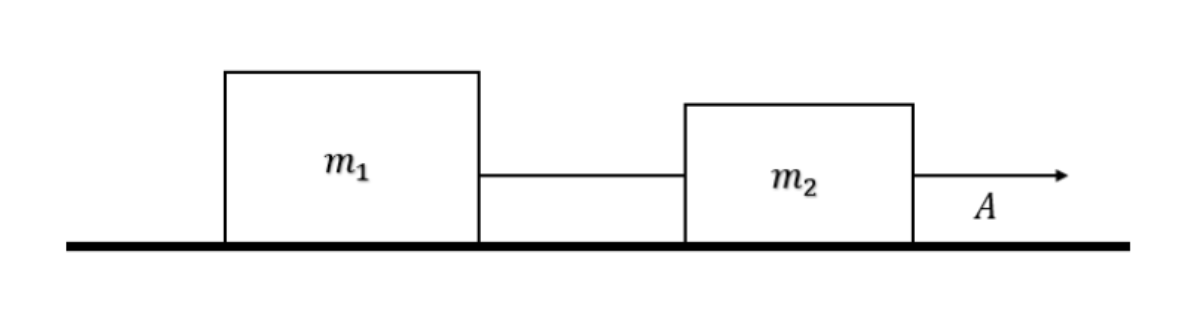
\includegraphics[scale=0.5]{Imagenes/Figura 1.png}
        \caption{Sistema de dos bloques amarrados}
        \label{fig:my_label}
    \end{figure}
\subsection*{Solución.}
Dado que hay dos cuerpos en el sistema, vaciamos las fuerzas que se ejercen sobre cada uno de ellos en dos diagramas de cuerpo libre:
\begin{multicols}{2}
    \begin{Figura}
        \centering
        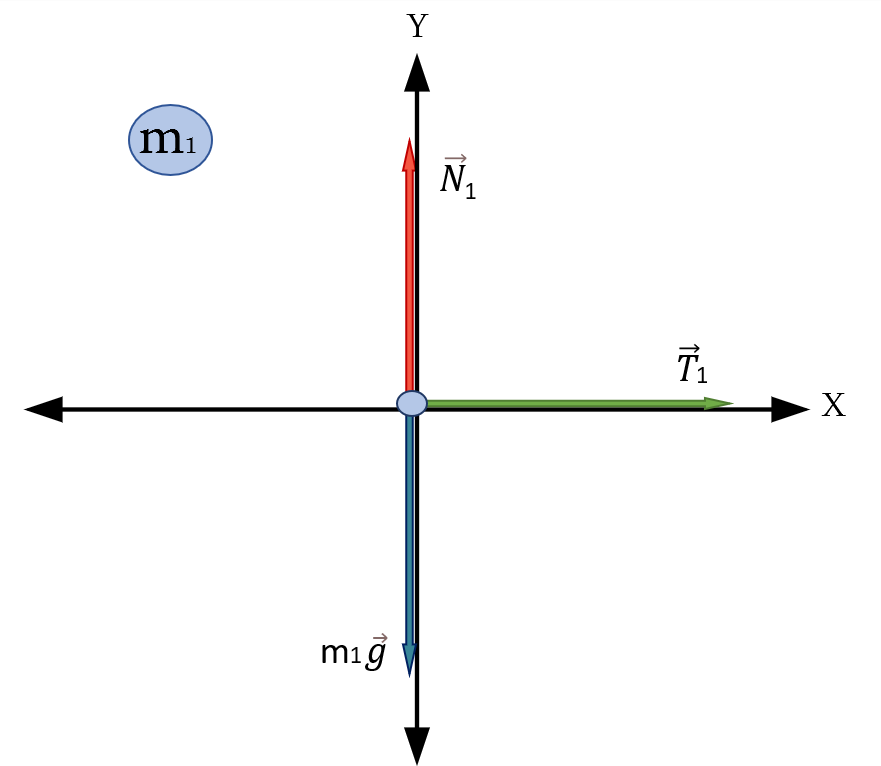
\includegraphics[scale=0.45]{Imagenes/DCL M1.png}
        \captionof{figure}{DCL de $m_1$}
        \label{fig:my_label}
    \end{Figura}
    \columnbreak
    \begin{Figura}
        \centering
        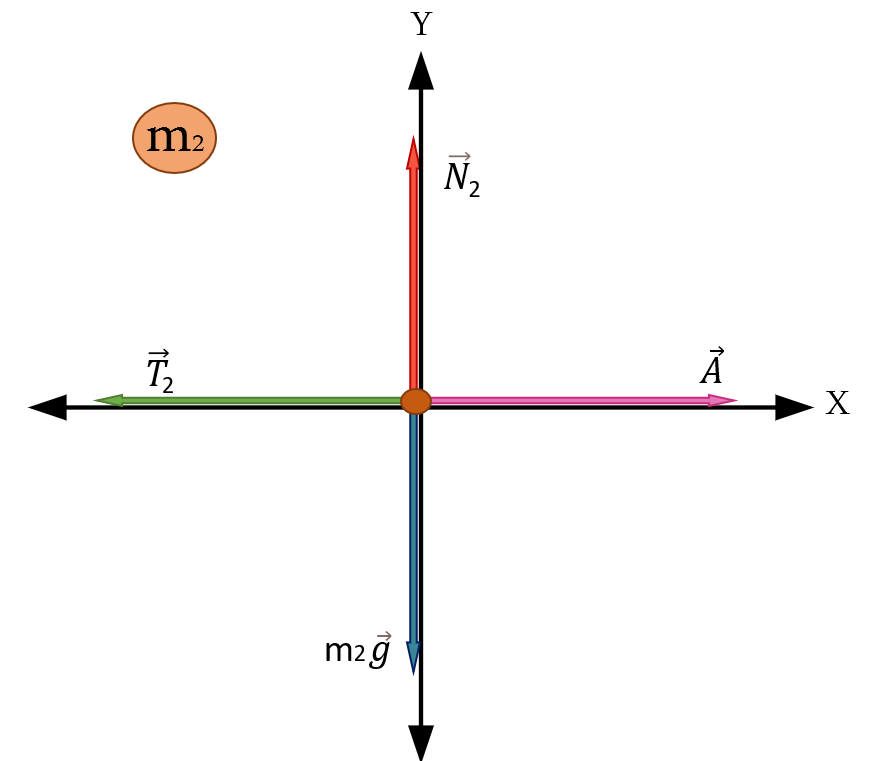
\includegraphics[scale=0.45]{Imagenes/DCL M2.png}
        \captionof{figure}{DCL de $m_2$ }
        \label{fig:my_label}
    \end{Figura}
\end{multicols}

\underline{Obs.} El problema menciona que la cuerda es ideal, por lo que es inextensible (no se estira) y no tiene masa, es decir $m=0$. Por lo que para cualesquiera dos fuerzas $F_1$ y $F_2$ se verifica que:
    \begin{align*}
        F_1 - F_2 &= ma\\
        F_1 - F_2 &= 0\\
        F_1  &= F_2
    \end{align*}
\hypertarget{uwu}{Así pues}, teniendo en cuenta que la tensión es un tipo de fuerza y de la observación anterior, decimos que $\vec{T_1} = \vec{T_1}$ en magnitud pero de sentido contrario. Por tanto, renombraremos a las magnitudes de las tensiones como $T_1= T_2 =T$

\underline{Obs.}Nótese que las fuerzas en el eje $X$ que actúan sobre $m_1$ y $m_2$ se equilibran, resultando $\Sigma F_y=0$, lo que provoca que no se muevan verticalmente, por lo que dichas fuerzas no interfieren en el movimiento del sistema y por tanto, sólo analizaremos las fuerzas del eje $Y$.

Ahora bien, por segunda ley de Newton, las fuerzas que actúan sobre $m_1$ son:
    \begin{equation}\tag{i}
        T_1 = m_{1}a \Longrightarrow T= m_{1}a 
        \label{eq:ec r}
    \end{equation}
Por otra parte, las fuerzas que actúan sobre $m_2$ son:
    \begin{equation}\tag{ii}
        A - T_2 = m_{2}a \Longrightarrow A-T= m_{2}a 
        \label{eq:ec ra}
    \end{equation}
Sustituyendo (\ref{eq:ec r}) en (\ref{eq:ec ra}):
    \begin{equation}\tag{iii}
        A - (m_{1}a)  = m_{2}a 
        \label{eq:ec raa}
    \end{equation}
Despejando a $A$ de (\ref{eq:ec raa}):
    \begin{align*}
        A = m_{2}a + m_{1}a\\
        A = a(m_{2} + m_{1}) \tag{iv}
        \label{eq:ec raaa}
    \end{align*}
Finalmente, despejando a la aceleración $a$ de (\ref{eq:ec raaa}) obtenemos que:
    \begin{align*}
        a=\frac{A}{(m_{2} + m_{1})}
        \label{eq:ec raaa}
    \end{align*}
    \begin{center}
        $\therefore$ La  aceleración del sistema  es $ a=\frac{A}{(m_{2} + m_{1})}$ y la tensión de la cuerda entre los bloques es $T_1= T_2 =T$ pero van en sentidos contrarios.
    \end{center}

    
    
\end{enumerate}



\section*{Punto extra}
Investiguen que hace la paquetería ``hyperref'' y expliquen que hace, citen su fuente donde fue investigado.
    \subsection*{Solución.}
    En general, la paquetería ``hyperref'' nos permite ``enmascarar un link'' mediante algún nombre que deseemos; pero también, es la paquetería que permite incluir links de manera explicita en el documento (sin nombrarlo de otra manera). Siempre que toquemos los objetos incluidos por ``hyperref'' nos direccionará al link que describe.
    La principal función de ``hyperref'', es que nos permite tener una tabla de contenido (índice) dinámica, en la que podemos navegar entre las diferentes secciones y subsecciones del documento mediante la asignación de ``hiperenlaces'' a objetos, redirigiéndolos a otra parte del documento. Sin embargo, estos objetos aparte de ser secciones, también pueden ser nombrados de distintas formas tal que direccionan a correos electrónicos, páginas de internet e inclusive permite conectar con servidores ftp y ejecutar aplicaciones (Overleaf, 2022)\\
    Estos hypervinculos pueden estar en cualquier parte del documento y pueden presentar o no un color de letra distinto (si es que el propietario del documento así lo desea) (Overleaf, 2022).\\

    Un ejemplo de este comando, se puede visualizar con lo siguiente:\\
    La palabra en color \href{https://www.youtube.com/watch?v=o_1aF54DO60}{\textcolor{blue}{azul}} , te llevará a un sitio web, mientras que la palabra en color \hyperlink{uwu}{\textcolor{red}{rojo}}  te enviará a una determinada página de este documento :)
    
\begin{thebibliography}{}
\bibitem{} Overleaf. 2022. \textit{Hyperlinks - Overleaf, Editor de LaTeX online}. \url{https://es.overleaf.com/learn/latex/Hyperlinks}.
\end{thebibliography}


   
\end{document}
